\section{System Design}
\label{design}

The Chimera system is divided up into a collection of components that
can be modified independently with little impact on the system.
{\em Figure \ref{design-figure}} shows these components and the points
of communication between them.
In this section, we will describe the various components
and how they interact with each other. We will also discuss the rational
between current design decisions and discuss some improvements that could
be made to the system.

\begin{wrapfigure}{r}{3.2in}
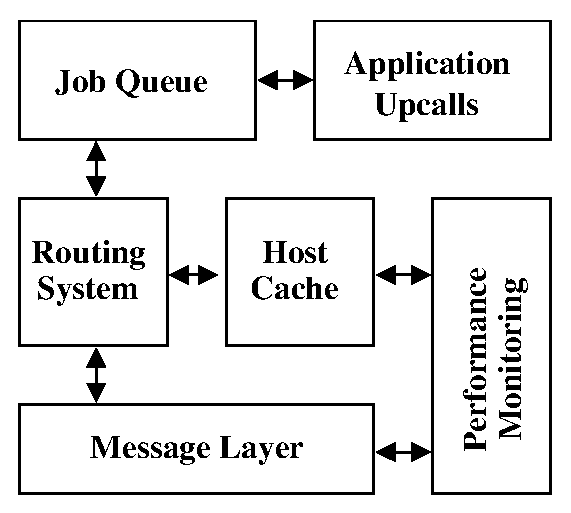
\includegraphics[width=3.2in]{design.eps}
\centering{\bf \caption{\label{design-figure} Chimera system design}}
\end{wrapfigure}

\subsection{Routing System}
\label{routing}

The core of the Chimera library is the routing system, which implements
a structured peer-to-peer overlay similar to Tapestry or Pastry
\cite{tapestry, pastry}. These algorithms are described thoroughly in
other papers, so we include only a brief overview of them.

A peer's routing information consists of two data structures: a leaf set
and a PRR routing table \cite{plaxtonnets}. The leaf set
contains the current peer's immediate neighbors in key space. This
leaf set is augmented by a PRR style prefix-matching routing table.
When a message arrives that needs to be routed, the local node checks
its leaf set
first. If the destination falls in the leaf set range, it will be forwarded to
the closest node in the leaf set. Otherwise,
it will be routed through PRR routing table to the node with the
longest common prefix with the destination.

Peers join the system by contacting a {\em bootstrap} node. After being assigned
a key, the node's join message is routed through the network to the peer
that will be closest in key space to the joining node. The 
joining peer then inherits
its initial routing information from this peer. Through the peer's lifetime,
it augments its routing information with peers that it interacts with or
learns about. Leaf sets are strictly constructed,
and must contain the closest known
peers in ID space for the system to work. PRR Routing tables have less
stringent requirements, and Chimera exploits this by updating this table
with nodes with the best expected performance. Performance numbers are
acquired through the {\em performance monitoring} subsystem.

This system is implemented using the soft-state mechanisms used in the
Bamboo system \cite{bamboo-churn}. This means that newly joined hosts are not
added to anyone routing table or leaf set until they have a complete
leaf set. Information about new hosts propagates relatively slowly, so
hosts are not likely to be found in routing tables until they have
been in the system a long time. Finally, operations performed
by the Chimera system are idempotent and non-atomic, so 
mid-operation failures can be handled by redundant messages without the
risk of putting the system in an unstable state.

The routing system is relatively complete, but there are many features
implemented by other systems that are lacking.
At the present time, keys for hosts and messages
are only 32 bits as opposed to the 160 bits most systems support. Also,
failure detection and recovery are fairly weak and could stand to be
improved. Specifically, the system could easily support multiple
alternate hosts for each PRR routing table entry, but currently doesn't.
There are many other improvements based on current research in the field
that could be added to the system.

\subsection{Message Layer}
\label{message}

Messages exchanged by the Chimera application consist of a message type, a
destination key, and the message payload. The type field is set either by
the {\em routing subsystem} or the application. Each message is handed off to
an upcall in the routing system which will do any processing necessary
and alert the application via upcall if requested. This effectively implements
an event-driven message passing architecture, where each message is processed
by an upcall at the receiving end. The key field is used
only for messages routed through the Chimera routing mesh, and may be
left empty for certain message types. The payload is the part of the
message that is delivered to the application.

Chimera communicates using UDP messages sent over BSD sockets. We implement
a simple, application layer network protocol on top of UDP to collect
feedback on message exchanges. Each network send made by the Chimera application
is assigned a monotonically increasing sequence number. This sequence number is
prepended to the communication, and the receiver responds with an application
level acknowledgement. If this acknowledgement does not arrive within a
certain timeout, the send fails.
In this case, the system may choose another valid route for the message, or it
may reissue the send to the same destination.
If the message is acknowledged, the communication time is recorded and sent
to the {\em measurement subsystem}.

The current message system is fairly primitive, and offers many opportunities
for improvement. For one, timeouts are currently statically determined, but could
be based on measurement information. Additionally,
this system could use failures in communication to detect host failures in
a more sophisticated way. Also, the
system currently treats each send as atomic, and if a send is not acknowledged,
it is cancelled and reissued with a new sequence number. By reusing sequence
numbers, it could be possible to be more tolerant of hosts whose responses
have been slowed by intermittent conditions.

\subsection{Host Cache}
\label{cache}

The host cache is used to maintain information on hosts that might be
useful to Chimera in the future.
The cache contains two data structures: a searchable list of all
hosts in the cache and an LRU list of hosts that are not currently in
use by the system. When a host is part of the peer's leaf set, PRR
routing table, or application data structure, it is locked into the
cache. When all references to the host are removed, it is appended to the
end of the free list. When a new host entry is requested, the host looks
for it in the cache. If it is found, it is removed from the free list if
necessary and returned. Otherwise, a new entry is created. If the cache exceeds
its maximum size, the first item is removed from the free list and replaced.
Otherwise, a new item is allocated. The cache is allowed to grow past its
maximum size if necessary, but it will try not to.

The host entries store both basic host information (name, address, key, port)
as well as auxiliary performance information. The main purpose of the
cache is to maintain this information even if the host is no longer actively
being used. A host that frequently communicates with a given peer will
likely have an entry in the cache. If another host fails and the peer needs
a new routing entry, it then has a collection of hosts with known expected
performance.

The cache is complete as is, but it identifies hosts by name and port only.
It would be more powerful if it was capable of searching for hosts
based on key.

\subsection{Performance Monitoring}
\label{performance}

The performance monitoring component is responsible for collecting and
reporting data on network conditions. This subsystem receives data from
the message layer regarding communication times and packet loss. It then
uses this information to update the host cache entry regarding the expected
performance of link to that host. Other components that access the host
entry can then use this information to make decisions based on the
expected performance of communication with a given host.

Currently, latency is determined using an exponential average of all
communication times seen. The current function gives 10\% weight to the
last measurement and 90\% weight to the measurement history
($m_{n+1} = (0.9 * m_n) + (0.1 * m)$). The loss ratio is computed using
the percentage of failed communications. These prediction mechanisms are
very simple and inaccurate, and in particular exponential averages produce
a highly varying prediction. There are more effective, but also more complex,
methods of predicting network performance.

\subsection{Job Queue}
\label{jobq}

In order to limit the number of threads that a program generates and
reduce the
cost of thread creation, Chimera creates limited
number of threads during the initialization phase. All these threads begin
as inactive, waiting for jobs to be submitted to the job queue.
As jobs are submitted to the pool, these threads wake up and begin to
process the job requests. If the number of jobs exceeds the number of threads,
they are put in a backlog and are processed in first-come, first-served
order.

It might be desirable to process jobs in a different order than simple
FCFS. In particular, it might become necessary to processes Chimera routing
messages with a higher priority than application messages. It might also
be simple to profile different job types and process them using an
approximate shortest job first schedule. However, until there appears
to be a need for these improvements, they will not be implemented.

\subsection{Application Upcalls}

Application upcalls are the method through which the Chimera system
interacts with the application built on top of it. In response to
certain events, such as message delivery, route requests, and leaf set
changes, the Chimera system calls functions provided by the user. The
user implements applications using these upcalls as described in work
on developing a common API for these types of systems \cite{commonapi}.
These upcalls are described more completely in section \ref{upcall-api}.

